\section{Introduction}

In this day and age, we collect a myriad of data about individuals, but these are not necessarily linked together. Merging survey data with administrative data is a recent trend, with American surveys leading the way (see Bates 2005, Dahlhammer and Cox 2007, Haider and Solon 2000). Even the panel ``Arbeitsmarkt und soziale Sicherung'' (PASS) from Germany which is annually conducted and executed by the Institute for Employment Research in Nuremberg, links survey responses to administrative records. The connection between survey data and administrative data lowers costs because researchers can reduce the length of the questionnaire. It also leads to more accurate data because often administrative data is more precise than the answers of the respondent. But with this method difficulties arise. For example, consent of the respondents is needed to merge administrative data and survey data. 

Because of the utility of linked administrative and survey data the way in which linkage for consent is asked has received a lot of attention. Researchers could put the administration linkage question in the back of the questionnaire because the question can be labeled as a highly sensitive or personal question. We see in the literature that sensitive questions are often asked at the end of the questionnaire to lower break-offs or unit nonresponse rates (Cantor and Cunningham 2002, Sudman and Bradburn 1982, Tourangeau and Yan 2007). In most of the American surveys the administrative linkage question is at the end. But German studies show that, in terms of consent rates, it is better to place the administrative question at the beginning (see Sakshaug et al. 2013). 

However, one can hypothesize the administrative data linkage question could lead to measurement error in later questions because respondents think that incorrect data can be corrected with administrative data (worse-respondent hypothesis). On the other hand, those who consent may be better respondents because they believe that their responses may be checked, and think they may get in trouble if they are found to be lying (better-respondent hypothesis). This change in reporting behavior due to the linkage consent question (if existing) can corrupt analyses. A higher share of worse-respondents for example could lead to higher share of measurement error which in return could lead to wrong inferences. Therefore we might either have a trade-off between a high consent rate and a possible measurement error or a win-win situation as the placement effect of the linkage question might obtain higher consent rates and reduces measurement error through better-respondents. This thesis tests the worse-respondent hypothesis against the better-respondent hypothesis.

For this study we have two datasets and the associated administrative data. The first one is conducted as a CATI\footnote{Computer Assisted Telephone Interview}. The second one is a follow up web survey that tries to recruit the telephone non-respondents. Both datasets contain an experimented manipulation of the administrative data linkage questions, one that is placed at the beginning and one that is placed at the end. The respondents were randomly assigned to one of these two conditions.

The aim of this thesis is to evaluate whether the linkage consent affects the accuracy of survey respondents' reporting. To answer this question.... 

\section{Background}
To address these two competing hypotheses about better- and worse-respondents I use three datasets -- two survey datasets and one administration dataset.  The administration data can be used as validation data to estimate the measurement error. 

\subsection{Administrative Data}

Over the last 20 years, Survey Methodologists have tried to make use of additional data. And that not only in social science survey but in a number of research areas. The English Longitudinal Survey of Ageing (Marmot et al. 2003) gathers samples of blood, genetic source material, records height, weight, grip strength and additional information about respondents' national insurance contributions, benefit and tax credit records.The Panel Labor Market and Social Security Survey (PASS) that is conducted by the Institute for Employment Research. This Panel uses the administrative data of the Integrated Employment biographies (IEB), which will be introduced later on. Using the linked administrative and survey data, additional analyses are possible that cannot be done of either datasets alone. 

To link administrative data with survey data has a lot of benefits. For one it can reduce costs because the questionnaire can be shortened. If there is already the information that is wanted in the administrative data, a question that asked the same fact is unnecessary. That would also decrease the interviewer and respondent burden (Sala et al. 2010) as the interview has fewer questions. Further we can assume that with linking, we get a higher data quality, because administrative data do not require the respondent. Respondents can, even unintentionally, make mistakes in their reports, because they are thinking of a socially desirable answer or do something wrong by retrieving the true value from their memory. Therefore studies often assume that administrative data is error free (Davern et al. 2008, Kreuter et al 2008, 2010, Sakshaug et al 2010). Administrative data often is compiled continuously and new information is added as soon as it is available  over a long period of time. That makes it a resource that is similar to panel data but much cheaper in production.

Linking the administrative data to survey data also has some difficulties. For one, consent of the respondents is needed to merge administrative data and survey data. Of course there are always respondents who exercise their right of refusal and do not consent. With the respondents having the possibility to non-consent, the linkage question produces an additional layer of non-response that threatens the quality of inferences (Sakshaug 2013). Furthermore, as studies that asked for permission for other personal data like administrative data and medical data have shown, those who consent and those who do not, can be quite different, leading to consent bias in linked data sets. These patterns of consent are not general and differentiate over studies and several variables (Haider and Solon 2000, Young et al. 2001, Banks et al. 2005, Jenkins et al. 2006, Dahlhammer and Cox 2007, Sakshaug et al. 2012, Dunn et al 2004, Huang et al 2007, Hartmann und Krug 2009; see Sakshaug and Kreuter 2012 for an extensive summary). 
 
That makes consenters non-representative for population statements (Jenkins et al. 2006). In addition, administrative data is gathered by the need of administrative processes and not for scientific research. Another problem is that research shows that there are inconsistencies between survey and administrative data (Sakshaug and Kreuter 2012). These inconsistencies can occur through errors in the record linkage process (Smith 2011) or through respondent difficulties in understanding the answer in some way that the administrative data generators do. 

As we see, research about the consent of the administrative data linkage question is still in the fledgling stage. One way to minimize the risk of high bias in inferences, obtained from linked data is to get high consent rates. Several studies have identified the design features of the linkage question that leads to consent. One way to do this is to adjust the wording of the question. Studies show that an indirect (Opt-Out) consent has a positive effect on the consent rates (Bates 2005, Pascale 2011, Das and Couper 2014), but many respondents do not seem to understand the subtleties of the question (Bates 2005), so it is hard to argue that this is a good method to obtain consent. Other studies show that the wording effect seems to be affected by the mode. While wording has no effect in CATI surveys (Sakshaug et al. 2013) it seems to work in web surveys (Sakshaug and Kreuter 2014). Another design features survey methodologists can account for is the selection of interviewers. These vary from study to study. Beste (2011) finds that interviewers who are female, older (+55) and have a low education achieve higher consent rates.  Other studies show that the higher the experience of the interviewer is the less likely they are to obtain consent (Sakshaug et al. 2013, Sala et al. 2010).

Another parameter that affects consent rates is the placement of the administrative data linkage question. Studies often put the administration data linkage question in the back of the questionnaire, because it is seen as sensitive. And as we see in the literature sensitive questions often placed in the later stage of the interview to lower break-off or unit nonresponse rates (Cantor and Cunningham 2002, Sudman and Bradburn 1982, Tourangeau and Yan 2007). In most of the American surveys the administrative linkage question is at the end, but it is better to place the administration linkage question at the beginning to get higher consent rates (see Sakshaug et al. 2013).

These results suggest that the administrative linkage question should be asked at the beginning of the interview to minimize the risks of high bias, when combining and analyzing the data. However when placed at the beginning, the administrative data linkage question may effect respondents' reporting behavior. This change in behavior can go in two possible ways. For one if the administrative linkage question is asked at the beginning of the interview, respondents could think that with the administrative data linkage incorrect data can be corrected. If they do so, they would take less care in their response and whether these are wrong (worse-respondent hypothesis)\footnote{A similar effect might occur with the interviewers: They could also believe that if they have the consent of the respondent, they do not need to read the questions accurately, because it may be corrected afterwards (worse-interviewer hypothesis) -- but we do not investigate this here.}. On the other hand, those who consent may be better respondents, because they believe that their responses may be checked, and think they may get in trouble if they are found to be lying (better-respondent hypothesis). This study tests the worse-respondent hypothesis against the better-respondent hypothesis. The hypotheses presented above lead to the main research purpose: to evaluate if the consent to the administrative data linkage question leads to a trade-off between a high consent rate and a possible measurement error or if this placement design leads to a win-win situation as higher consent rates can be obtained and measurement error can be lowered.

\subsection{Response process - The hypotheses in context of the general response model}


The cognitive process of answering a survey question has four steps: a) Comprehension, b) Retrieval, c) Estimation and Judgment and d) Reporting (Tourangeau et al 2000, Dillman et al. 2009, Groves et al. 2009). In the first step -- comprehension -- the respondent is encoding and interpreting the question in the survey context and tries to figure out what exactly is wanted from him/her. In the retrieval step, the respondent tries to remember the information that is important to answer the question, such as facts, memories, events and so on. When the respondent is in the state of Estimation and Judgment, (s)he is thinking if the retrieved answer is right, accurate enough or can be mentioned in the context of the interview. At the end of the process reports his/her answer. 

The response process is not necessarily linear but a process that can skip stages and contains overlaps between the stages. In fact many things can go wrong. In the comprehension process. Respondents may not notice introductions to the question or do not bother to read them. Further they can run across unfamiliar terms or the question requests detailed information that the respondent does not have. One major problem in asking questions is the different meaning that researchers and respondents have about a specific term (Tourangeau et al 2000). 

To understand how errors are involved in the retrieval process, we first have to understand how this process actually works and how the respondent gets the information needed. Memory is not organized in a stream of isolated events but in a bundle of temporal-causal sequences (Sudman et al 1996). To get at the wanted information, retrieval cues are used (Groves et al 2009). We should imagine these as a huge network of information whereas the cues are the roads that connect the stored memories. These cues help the respondent to structure the memory, events, facts etc. with the result that they might find the right answer. Cues are usually provided by the question itself. Mentioning the first cue leads to another cue and so on until the respondent finds the needed information.

This process can be really long and hard for the respondent so that (s)he might give up before the right answer appears. Moreover whenever €œthe cues provided by the question do not match the information actually stored in memory, retrieval may fail€ (Groves et al 2009). 

In fact remembering an event is not a direct retrieval but the result of inference or reconstruction (Bradburn et al. 1987). Because of the structure of the retrieval cues, we do not have exact dates and linkages that are saved in our memory but more of a structured overview. The remembered memories, events and facts are not quite exact, and the respondent has infer or reconstruct parts of the event, memory or fact. Therefore the line between retrieval, inference and reconstruction blurs (Tourangeau et al. 2000). It is the Judgment and Estimation of the respondent who decides that the found answer is correct or correct enough.

The cues that are responsible for the judgment about the response are identified by Cannell et al. (1981): the respondents' choice of response is based on cues from, a) the interviewer's status, appearance, gender, age and behavior, b) the question and the preceding questions and c) the respondents' beliefs, values and goals. All these cues can lead to the respondent editing his\textbackslash her response because of social desirability and self-presentation (Cannel et al. 1981, Sudman et al. 1996)

At this point we can return to the hypotheses about the response behavior of the respondents. We hypothesized that consenting to the administrative data linkage question that is asked at the beginning of the interview can lead to better-respondents because they might believe that their answers may be checked and that they would get in trouble for misreporting. Alternatively worse-respondents who could believe that most of the information is already there and misreports may be corrected by the researchers. With our hypotheses and Cannell et al (1981) question cue, we locate the reason for a possible response bias: consenting to the linkage question asked at the beginning of the interview changes the context of the following questions and generates a response bias for these. 

In a general survey setting we should be able to control some of the errors mentioned above and some not. There will be respondents who do not care and invest less effort in answering the questions of the interview. In fact respondents are `cognitive misers' (Fiske and Taylor 1991). Krosnick (1991, 1999) extends this approach and distinguishes between optimizers and satisfiers as respondents who answer questions. Optimizers are respondents who put a high effort and diligence in answering the questions in an interview. Satisfiers on the other side put the least effort into the four step process mentioned above. Those are the respondents who are inattentive as reading or hearing the question or ignore further introductions. They may skip the retrieval stage or do not recall all information needed and just use the least effort to give a plausible answer.

Optimizers and Satisfiers are both the termini of a continuum (Krosnick 1999). Both are ideal types and should not exist in there full might; at least there should be very few of these extreme types. Anyway every respondent is located somewhere on this continuum. 

The basic attitude (beliefs, values and goals) that determines the initial location on the optimizer-satisfier-continuum should be stable for each respondent in the pre-interview situation. Also I assume that the basic attitude determines the effort that respondents put in the cognitive response process. With the consent to participate in the interview, the respondent is exposed to several cues like interviewer characteristics and questionnaire design that should motivate most of the respondents to move from their initial location. I hypothesize consenting to the administrative data linkage question at the beginning of the interview changes the motivation of the respondents so that they leave their initial location on the optimizer-satisfier-continuum. In this sense, the linkage question can be seen as a treatment. The question is if the effect of this treatment is perceptible in the data and in which direction it goes, because respondents can be motivated to give better responses as or they could give worse responses. It is not clear how the administrative data linkage question motivates the respondents to move on this continuum, but a general tendency should be perceptible if we aggregate the responses.
	


There are two different ways how the treatment effect of the administrative data linkage question could work out. For the better-respondent hypothesis the treatment could lead to the motivation of the respondents to answer more accurately and therefore the measurement error of the treated group should be lower as if they would not have been treated. For the worse-respondents who put less effort in answering the following question through consenting to the administrative data linkage question the measurement error should be higher as if the respondents would not have got the chance to answer the linkage question.

\section{Data}
\subsection {Survey data}

To tackle the research question it is possible to use a survey that is conducted by the Institute for Employment Research (IAB). This mixed mode survey was designed to investigate different methods of protecting individual privacy and transferring addresses to survey firms for data collection purposes. The IAB selected a random sample of 17,001 persons from the Integrated Employment Biographies data (described in more detail below). The survey took place from the 9. October to the 31. Decemeber 2014.

This survey is conducted as a two step mixed-mode survey. First a computer assisted telephone interview survey (CATI) was performed. From 7,183 eligible cases 1,208 could be interviewed. Therefore we have an overall response rate of 21.3 \% (APPOR RR1). Second, as not all selected cases could be interviewed because they denied the address transfer in the prior experiment\footnote{For more information about this experiment see Appendix \ref{sampling}, p. \pageref{sampling}.} and non-response the same survey was shortened and performed as a web survey. Overall 1,090 of 9,607 eligible cases completed the web survey. The response rate is 11.3 \% (APPOR RR1).

Both surveys contained experiments that evaluate the effects of wording and placement of the administrative data linkage question on consent rates. 

\subsection*{The linkage question}

The Survey described above included additional experiments with wording and placement of the administrative
linkage question.  The respondents were randomly assigned to one of four conditions. Two conditions asked the linkage question at the beginning and two at the end. Respondents were also randomized to receive one of the two wordings. The first wording was formulated in a gain frame: the wording focused on the benefit for the study if the respondent would consent. The second formulation was in a loss frame, where the focus was on loosing some benefits of the study, if the respondent denied linkage consent. The remaining wordings of the questions were read the same. 

Table \ref{tab:consentrates} gives the achieved consent rates in each of the four conditions for the CATI survey. To ask at the beginning seems to conduce to a higher consent rate. Also the wording seems to have no effect on consent rates. These results are in line with other studies that already explored placement and wording of the administrative data linkage question (see Sakshaug et al. 2013).

In the web survey the consent is with 76.71\% lower than in the CATI survey. Also we can
see differences in the single questions. Again it seems better to place the
administrative data linkage question at the beginning of the questionnaire rather than at
the end. Also this time the wording seems to have an effect on the consent rates. As we see in Table \ref{tab:consentrates} the loss frame wording gets at the beginning with 86.31\% and also at the end with 75.40\% a higher consent rate than the gainframe wording. Sakshaug et al. (2013) show similar results in their study.


In terms of maximizing the consent rate, asking the linkage question at the beginning seems to be a good idea in both modes. Thus the research question applies to both modes because the trade-off between a higher
consent rate and a possible measurement error is constituted. But as the reader will have noticed there is also a mode effect. While CATI respondents seems to be unaffected by wording, it has a rather high impact on respondents in a web survey. Thus in answering my research question, I separately account for the two modes. However because the wording seems to only have an effect at the end of the web survey, I do not explore the effect of wording on measurement error. Though that must not be true. But for the restriction of space in this study, I cut it off. It has to be evaluated in further studies.


\subsection{Administrative data}\label{admin}

I link the survey data described above to administrative data to get additional data for our analysis. The administrative data being used for this study is the Integrated Employment Biographies (IEB). This data displays the complete employment biographies of persons in working age that are reported at the Federal Employment Agency. To get the data the IT- and Information Management of the Institute of Employment Research combines a set of standard data products that are available at the Institute for Employment Research. These data products are history of employees, measures of participation on the labor market politic, history of benefit recipients, history of benefit recipients basic security and job seekers. To merge all the needed data to gain the Integrated Employment Biographies data the ITM uses an overall person identifier to generate a standardized statistical person. The administrative data I use contains information on employment, receipt of both types of unemployment benefits (SGB II and III) and the participation on measures of active labor market politics since 1975 for all persons in the survey's sample.

The data contains characteristics of persons such as date of birth, vocational training, gender and residence. Also it contains data specific characteristics like job location, economic sector and active labor market activity. But the data is also restricted because it only contains variables that the Federal Employment Agency needs to calculate pay dues into the unemployment insurance and claims in the case of unemployment. For example calculating net income is difficult because variables like tax category, number of kids and marital status are missing (see FDZ-Methodenreport 13/2014:6). 

Variables that are in the administrative data but have a high share of missing values are the education variables, because the educational status is not needed for administrative processes and no consequences appear for employers and employees by not stating it (Fitzenberger et al 2005). Since these variables are needed for the analysis I impute these with the imputation rules (IP 1) of Fitzenberger (et al 2005). to account for the missing data.

The data, are updated once a year. For this study it is possible to use the IEB data from the 31. December 2013, which is nine to twelve month prior to the date of the survey.

As the survey data is from the end of 2014 and the sample is selected from the administration data that is from the end of 2013, we cannot easily compare these two data sets. If a researcher, for example, wants to find out if there is some misreporting in the employment status of the respondents, (s)he cannot compare the last statement in the administration data with the statement in the survey data because the moment is different. Probably there may be a mismatch between the two data, because of job changes over time. One could assume that these mismatches are randomly assigned over both groups and that there should not be an effect on the comparisons because it is constant. Anyway, this is not good enough. Luckily the administration data has spells of each person, that gives information about the period of employment, unemployment etc.

Spells are units that structure the Integrated Employment Biographies. They are periods that contain the data about employment, unemployment, job seeking, benefit receive etc. Each person has spells from his/her entry in the labor market to his/her current employment status. For each new employment status, change in amount of benefit receive, salary or job change etc. a new spell will be generated. With that a time line for each person of his/her personal employment biography can be drawn and it is possible to compare the moment of the respondents statement with the administrative.

To compare moments from the survey with spells is not easy either because the transition of spells is not stringing together. We can distinguish the transition of spells in three categories: flow, overlap and gap. Flow means that the transition from one spell to another is a one day break. This happens for example if the employment contract ends and a new employment contract begins on the next day. It would also be possible to go directly to an unemployment spell after the employment contract ends. To have a flow between spells is possible but unlikely. Most transitions have a gap, at least a short one of a few days. That means that between two spells lies an unobserved period. This happens because of various reasons. The next employment could start after a month of the last employment, the person could miss it to request unemployment benefits in time, the person could start a work as an official or self-employed or is basically not eligible for benefits, for reasons whatsoever etc. Last but not least we have overlaps of spells. That happens if people have two jobs at the same time or have a job but also qualify for benefit receipt.


\subsection{Merging the survey data with the administrative data}\label{mergeing}

exact linkage. This method should obtain the highest and most exact linkage rate. But it is not error free and the possibility of wrong matches exists. Further a few adjustments have to be made for this study to ensure internal validity.

Due to certain characteristics of the survey and administrative data, I have to drop several cases before starting the analysis. The cases I drop are non-consenters, wrong matches, incompletes, officials and self-employed persons. Table \ref{tab:loss of cases cati} shows a summary of all cases I drop. As we need consent of the respondents to merge the administrative data with the Survey data, we cannot merge the non-consenters: 178 cases in the CATI data and 316 in the web data.
	
	Further as the administrative data is process data and changing over time it is possible that the personal identification number changes too. For the identification of the persons gender and the year of birth was used. So everybody who has not a match in these two variables between the administrative and survey data is considered a wrong match. For the CATI data we have four people that do not match in gender and 15 that have a different year of birth. For the web data we have 43 cases that either have not a match in year of birth or gender or both. 

\begin{table}[h]
	\centering
	\caption{Loss of cases through calculating the measurement error the variable employment status with the begin dates}\label{tab:loss of cases}
	\begin{tabularx}{\textwidth}{Xll}
		\addlinespace \addlinespace
		& CATI & web \\ 
		\midrule
		\addlinespace
		Starting sample size		&1,208&1090  \\ \addlinespace \addlinespace
		Non-consenters				&178&316 \\ \addlinespace
		Wrong matches				&19&43  \\ \addlinespace 	
		Incompletes 					&66&40    \\ \addlinespace
		Officials and self-employers&38&142    \\ \addlinespace \addlinespace
		Final sample size			&917&585   \\ \addlinespace	
		\bottomrule    
	\end{tabularx}
	\small
	\begin{tablenotes}
		\begin{footnotesize}
\item Note: Please acknowledge that there are overlaps between the groups of wrong matches, incompletes and officials and self-employers
		\end{footnotesize}
	\end{tablenotes}
\end{table}

	Officially the administrative data goes until the 31.12.2013. As the data is extracted, it is possible that not all spells are available because institutes fail to report them. It is common practice to add these missing spells in the follow up years. Therefore we have cases that have an incomplete number of spells. From this it follows that these cases do not have an end date that equals the 31.12.2013 or later. I top code the analysis to this date. We have missing periods that we do not know anything about for every person that has not a spell that goes until this date. So I take these cases out so that they not bias the analyses. In total 66 cases are incomplete for the CATI and 40 cases for the web data. This may not seem reasonable at the time but will be explained later on as the variables will be presented (see section \ref{variables}, p. \pageref{variables}). 
	
	The last group we cannot analyze are the respondents that stated to be an official or self-employed. About this group of persons the administrative data has no information because they are not subjects to social insurance contributions. In the CATI data total of 38 cases stated at least in one of the three loops that asked for employment status that they were an official or self-employed. For the web data we have and bigger loss as 142 respondents stated that they were officials or self-employed.
	
	Overall we have a final sample size of 917 respondents what makes a lost of around 24\% of the actual sample size of 1,208 cases. In the web survey the loss of cases is even bigger. Around 46\% of the actual sample size (1090 cases) get drop out because they cannot be analyzed. 
	









\section{Method}\label{method}

To study the effect of the administrative data linkage question on response behavior, I use techniques of causal analysis. 

\subsection{Counterfactual Causal Model}	

To estimate the effect of the linkage question on response behavior it would be the best, if we knew how the respondents would have answered if they had not been asked. Such counterfactual outcomes are not available because we can not observe that. Therefore we have to construct a replacement for the counterfactual outcomes to check the effect of consenting to the linkage question. 

One possible solution would be to compare the consenters against the non-consenters. The Non-consenters are not exposed to the effect and therefore should be a good counterfactual group. Since we have a survey experiment were the respondents are randomly allocated to the linkage question at the beginning or at the end of the questionnaire, we have a large group of respondents that did not got the linkage question at the beginning. These are also not exposed to the effect and might be suitable as a counterfactual group. 

Both solutions lack some requirements. To estimate a change in response behavior I use the change in measurement error as an indicator. The measurement error is calculated from comparing the values of the survey data with the values from the administrative data. As I do not have any individual-related administrative data for non-consenters, I cannot calculate the measurement error for those. Therefore I cannot use non-consenters in the analysis. 

The second approach -- using the respondents that got the linkage question at the end of the interview -- has the same limitation in terms that there are non-consenters in this group, which cannot be analyzed. That leaves the possibility to compare the consenters from the beginning with consenters from the end. But that would be a rather naive estimation. 

To declare a group as a suitable counterfactual group, the counterfactual group has to be equal distributed characteristics to the observed group. Since we have consenters, we have a decision, be it conscious or not, who select themselves to be in a treatment group. Although the respondents were randomly allocated to get the linkage consent question at the beginning or at the end, these who gave consent at the beginning are different than these who gave consent at the end. To estimate the true effect of the linkage question, one has to account for this selection bias and isolate this effect. Therefore we need to achieve balance of the covariates between both groups to simulate a randomized distribution\footnote{Selection bias applies for the first solution too. Even if we had individual related administrative data for non-consenters, we have to assume that both groups differ from each other.} and be able to calculate the `true' treatment effect.

\subsection{The entropy balance scheme}

There are several techniques that are named under propensity score matching, which are used in observational studies estimate the `true' treatment effect (Altonji et al. 2005, Morgan 2001). All techniques share the same basic approach to control a set of observed covariates (X). 

If one wants to match or balance out two groups over a set of covariates it is hard to do it over an exact matching. Instead we will use a technique proposed by Hainmueller (2012) called entropy balance. Entropy balancing goes the reverse way of the propensity score reweighting. With the reweighting method researchers calculate unit weights with a logistic or probabilistic regression and then check for balance. Entropy balance estimates the weights for the control group cases directly from the imposed balance constraints (Hainmueller 2012). These balance constraints are three moments: mean, variance and skewness. For this thesis I control the first moment constrain, the mean. To control higher moments reduces the chance of the entropy balance scheme to achieve convergence. In addition, controlling the mean as a moment constrain is often sufficient to balance out the variance and skewness as further moments too (Hainmueller and Xu 2013).   

If the propensity score model does not work because the model is misspecified, researchers have to readjust the model and do the same process again until it works. Entropy balance on the other side takes this burden from the researcher (Hainmueller 2012). 

To have balanced covariates between two groups the literature relies on three assumptions: the Stable Unit Treatment Assumption Value Assumption (SUTVA), the conditional independence Assumption and the overlap assumption. 

The Stable Unit Treatment Value Assumption implies that the cases do not depend on each other in terms of who is in the treatment group or how large the treatment group is (Eckman/Nichols 2015). It assumes that there are no spill-over effects and that responses are not dependent of the response of other units (Rubin 1980, Holland 1986). 

The second assumption is the conditional independence assumption\footnote{In the literature you can find different terms for this assumption: ignorable treatment assignment (Guo and Fraser 2015), unconfoundedness (Rosenbaum and Rubin 1983), selection on observables (Barnow et al 1980), conditional independence (Eckman and Nichols 2015), exogeneity (Imbens 2004), sensitivity analysis to assess the plausibility (Stuart 2010). All mean the same. For this thesis I use the connotation of conditional independence.}. It assumes that a set of covariates \(X_{i}\) is not affected by the treatment (Caliendo and Kopeinig 2005).

Third assumption is the overlap assumption. This assumption implies that in the treated and in the control group are persons with identical characteristics (Heckman et al 1998). That means for all covariates (X) must be a positive probability to one of both groups because is there a covariate that is either treated or non-treated the persons cannot be compared. 

In observational data, as the data I use is, these assumptions are not covered and I would compare groups that are not randomized. Therefore I would have a bias in the estimation of the treatment effect. With the entropy balance scheme I simulate a randomized assignment. 

Because we cannot observe any important variable, we cannot adjust all covariates. To fulfill the conditional independence assumption it requires to have all covariates observed that influence the treatment assignment and the outcome. This assumption to have no unobserved differences between the treatment and control group is also called strong ignorability (Stuart 2010, Eckman and Nichols 2015) but this is not testable tough (Imbens 2004). This approach is therefore an approximation to the randomized allocation. But usually it is assumed to have all important covariates covered. 

\subsubsection{Covariates for balance}\label{covar}

To regain balance between the treatment and the control group to simulate a randomized distribution between both groups it is important to include all known variables that are related to the treatment assignment and the outcome (Stuart 2010 Eckman and Nichols 2015). Including all available covariates makes it more likely that the strong ignorability assumption is satisfied. Further the listed variables presented below have not consequently an effect on the treatment assignment or outcome, at least not one that is viewable immediately. Here I follow the kitchen sink approach (Eckman and Nichols 2015), which recommends to take all available variables into account. Indeed variables that are unassociated can increase the variance of the analysis but excluding important variables can increase the bias (Stuart 2010). 

For our model I use mostly variables from the administrative data, because it is the hypothesis of this thesis that consenting to the administrative data linkage question has an impact on the response behavior. Therefore the survey data after the administrative data linkage question may be corrupted. If we would balance the treatment and control group on variables in the survey data, we would get a treatment effect of zero because all possible effects are balanced out. In fact to balance both groups and keeping the effects of interest we have to exclude any variable that may be affected by the treatment of interest and use only variables that are fixed over time or measured before treatment (Rosenbaum 1984, Frangakis and Rubin 2002, Greenland 2003, Eckman and Nichols 2015, Caliendo/Kopeinig 2005).

Because of his\textbackslash her structure the administrative data is not immediately usable for the entropy balancing model. The needed variables have to be computed from a process to a time-moment structure. For this study I support the variables being used through the fact that they were already used in a previous study that obtained balance between treatment and control group with a propensity score reweighting model (Bach 2015).

The variables are summarized in Table \ref{tab:covariates}. Variables among others which are included in this model are year of birth and gender. Both variables were used as a verifier to determine the right respondents and asked before the linkage question. Therefore if year of birth and gender do not correspond between administrative and survey data I assume a wrong match and exclude these cases from the analysis (see \ref{mergeing} Merging the survey data with the administrative data, p.\pageref{mergeing}) So those two variables are not corrupted by administrative data linkage question and can be applied to the model. Further variables are the education and the west/east variables.



Next to sociodemographic variables, the administrative data provides a number of Labor market history variables. For every person we can calculate the mean duration, total duration and the number of spells for the unemployment benefit receipt I and II, ALMP participation, Employment, Unemployment and Job Seeking. With these variables are some facts to mention. As told before the administrative data is organized in spells. Every time something employment related does change in the live of a person, like a change of income or the amount of benefit receipts a new spell is added. So with any change within one of the six presented categories above the mean duration of that person in that category drops because it is calculated from the total duration and the number of spells of the same category. Therefore: the higher the change within the category the lower the mean duration. Normally this would be a problem as these variables have a high bias. But since it is our aim to regain balance and therefore to predict a right weight for each case to get that balance, we do not need to interpret this model and therefore these variables do not need to be interpretable. Instead we assume a randomized distribution for the variables weakness over all cases. 

Another variable being taken into the model is the share of different employers to the time of extraction of the administrative data.

Other variables that should join the entropy balance model is the sample selection and the loss/ gain-frame experiment of the administrative data linkage question. 

A last group of variables I include to the entropy balance model are interviewer characteristics and call record data. These variables can only be included in the entropy balance model for the CATI data. For interviewer characteristics age, gender, education and interviewer experience is included. For the call record data the number of contacts and the contact time serve as indicators. Interviewer characteristics are known to be related to nonresponse (Groves et al 1992, Groves et al 2000, Sinibaldi and Eckman 2015). As interviewers are randomly assigned to the respondents these variables seem not important because we have no information about non-respondent. But as mentioned in the background section, the administrative data linkage question can be seen as a second layer of non-response (Sakshaug 2013). Also Interviewer characteristics can impact the respondents' decision to consent to the administrative data linkage question (Beste 2011, Sakshaug et al. 2013, Sala et al 2010). For the Call record data we know that hard to get respondents can differ in their responses from the respondents that are easy and earlier to interview in the field period (Kreuter et al 2014).

To test if the covariates are really balanced out I check the standardized mean differences. To evaluate the standardized mean differences as sufficient a deviation up to five percent is decent (Caliendo and Kopeinig 2008). Therefore every entropy balance model that has a deviation of the standardized mean differences over five percent is labeled as non-working. 

\subsection{Treatment Effect Estimation}

Further I evaluate the treatment effect for several variables each variable we have a different amount of cases. So basically we need to rerun our method to regain balance for each variable.

To estimate the treatment effect I use simple regression models with the treatment indicator as the independent variable, the weights from the entropy balance model applied and robust standard errors. Since I evaluate the effect of consenting to the linkage question at the beginning of the interview on the measurement error most variables are binary coded  (\(0=true\ report, 1=false \ report\)). Therefore I compute regressions with two binary variables. Usually that is bad style. In this case it seems to be a good and also better choice than a probabilistic regression that is usually used with a binary outcome because the interpretation is easier. 

The weights for the regression model are calculated from the entropy balance model I presented. The entropy balance model calculates weights for the control group so that they equal the treatment group. If I proceed like this, I calculate the average treatment effect of the treated (ATT). This one measures the increase of the outcome variable due to receipt of treatment among those who choose treatment (Eckman and Nichols 2015). The average treatment effect of the treated is the most common in observational studies because most treatments rely on a decision like the decision to attend college or not. However, as related to this thesis if we would estimate the average treatment effect of the treated it would be like as we compare the consenters and non-consenters of the administrative data linkage question at the beginning of the interview because the respondents decide to be in the treatment group.

Ideally I would prefer to estimate the average treatment effect (ATE). This effect measures the expected effect if the respondents were randomly assigned to the treatment and control group (Caliendo and Kopeinig 2008). It is theoretically possible to balance the covariates for average treatment effect estimation with an extension of the entropy balance scheme (Hainmueller 2012). But the presented technique from Hainmueller (2012) can so far only weight the covariates for the estimation of the average treatment effect of the treated. It is not the aim or task of this thesis to develop this method. That is a job for coming research. Therefore I need another approach. I stress the fact that the average treatment effect of the treated equals the average treatment effect by randomized allocation. 

Equation \ref{eq:ateequals} is only true under the assumption that treatment and control group are randomly allocated (Eckman and Nichols 2015, Wooldridge 2010, Angrist and Pischke 2009). As I mentioned before both groups are not randomly assigned but suffer from selection bias. But with the entropy balance technique treatment and control group are both balanced out and a randomized assignment is simulated under the assumption of strong ignorability\footnote{All important variables that have an effect on the outcome or treatment assignment are known and observed.}. That means if the model presented above is specified in the right way it should hold that ATT=ATE. 





\section{Dependent variables for the treatment effect estimation}\label{variables} 

I present the dependent variables for the regression model that I use for my analysis. This thesis cannot test all existing variables in the data. The reason therefore is that the data structure for questions asked in the survey is not equal to the data structure of the administrative data. Therefore adjustment is necessary and the analysis is limited on a few variables. In the following I present the items of interest: employment status, begin of employment, nationality and income. There are differences in terms of number of analyzable variables between the CATI and web survey because the latter is shortened. According to the hypotheses the measurement error should increase for the group that consented to the linkage question at the beginning, because respondents care less about accurately answering the questions (worse-respondent hypothesis). If the better-respondent hypothesis applies the measurement error should decrease because respondents may take more effort to answer the questions.    

\subsection{Employment variables}

For the CATI data there is information on up to three jobs available. The respondents were asked what their current employment status is. After answering this question a series of follow up questions were asked. Among others the begin date of the current employment status was demanded. If the respondents did not state a begin date before 01.01.2010 they were put in a loop and asked what kind of employment status they had before their employment status that they stated. They were also asked all follow-up questions about their employment status including the begin date of employment, if they were employed. Overall there were up to three loops possible under the condition that their employment status of interest did not begin before 01.01.2010. 

For the web survey the employment-status and follow up questions were only asked one time.
  
I focus on two employment variables and their peculiarities. The first one is the employment status and the wording can be found below\footnote{Translation from author.}:

I recode this question to a binary variable whereas employed is still classified as employed and all other categories are classified as non-employed (except for do not know and no answer, these are missing values). After this question a number of other questions followed to get information about the period of employment or unemployment. 

I check with the administration data if the respondent misreports about his\textbackslash her employment or not. As follow up questions come with each statement, respondents should learn to avoid the cognitive effort by misreporting about their employment for each loop (Eckman and Kreuter 2015). If we remember the worse-respondent hypothesis, respondents that consent at the beginning should care less about answers and may misreport. Better-respondents on the other hand should give more accurate answers. Therefore, concerning the research question, there should be a difference between the consenters at the beginning and our constructed counterfactual group.

There are certain problems, if one wants to compare the employment status from a survey with the employment status from the Integrated Employment Biographies data. As written before the administrative data is structured in spells about employment and unemployment periods. Their transitions can be categorized in flow, overlap and gap (see \ref{admin} Administrative data, p. \pageref{admin}). These different kinds of transitions make it really hard to compare the values because we can not just take the current spell and compare it with the answer of the first loop. We could get a benefit drawing spell but actually the respondent is employed of a minimum wage basis. And it gets even harder if we go back in the past\footnote{The Respondent could give information about a gap that we will miss. If two jobs overlap, we could get one job in the first loop and the other one in the second. But the Respondent was told to mention the job with the highest salary. So for the first loop we get that job. But what if the second job with the lower salary started before the job with the higher salary. Does this respondent in the second loop mention the job with the lower salary or does (s)he mention the period, be employed or unemployed, before he got one of those two jobs? We could make assumptions about it and live with a bias that we assume is balanced over the treatment and control group.}.

Another problem is that we cannot account for progress in the job. For example a person begins his\textbackslash her employment as an intern. After that (s)he gets a full-time employment with a flow transition. For the next ten years until today (s)he gets promoted four times and becomes a new employment position with another role, tasks and maybe another job location within his\textbackslash her establishment\footnote{Please remember that every time something changes in the job situation of a person a new spell will be generated}. If we ask, whether this person is employed or not, we can approve that (s)he is. But when did his\textbackslash her employment actually start: with his\textbackslash her internship, the begin of full-time employment, the last promotion or anything in between? For the purpose of this research question, we could say that we state a general interpretation for the begin of employment, collapse these spells, do the analysis and live with the bias that comes with it. 

There are various other combinations of biographies. This thesis cannot explore or account for all of these combinations by collapsing and sorting the spells from the administrative data. Fact is that there is a huge room for interpretation for the respondents to answer in the loops. If we collapse and sort the spells, we get messed up data and analyses. Therefore we have to approach differently.

To figure out if the Respondent stated the right employment status to the time of the interview, we use the begin date of his\textbackslash her current employment status. For each category that the respondent could choose for their employment status, the begin date was asked too. That means there should be no change in employment status after the date in the first loop or between the second[third] and first[second] for the second[third] loop\footnote{For more information about how the measurement variables are calculated see Appendix: \ref{calcME} Calculation of the employment measurement error variables, p.\pageref{calcME}.}. If there is a change, I assume that the respondent misreports about his\textbackslash her current employment status.

The second question of interest I focus on is a follow up question about the start date of the employment: 

The respondents had the chance to state the month and year of the begin date. To calculate the measurement error variable, I take the minimum difference between the date stated in the survey and the dates in the administrative data employment spells as the deviation from the true score\footnote{For more information about how the measurement variables are calculated see Appendix: \ref{calcME} Calculation of the employment measurement error variables, p.\pageref{calcME}.}. The deviation is an absolute value \((\Delta_{begin \ date}\geq0\)) to ensure that negative and positive deviations do not cancel each other out in the analysis.

For respondents exact dates are the hardest to remember (Wagenaar 1986, Friedman 1993). Luckily the respondents had only to remember the month and the year. Also with the increase of time an event happened the more accuracy decreases (Cannel et al. 1981, Loftus et al. 1992, Means et al. 1989). Anyway, as begin of the employment is further in the past with each loop, it is hypothesized, that measurement error in general should increase. Also the cognitive effort should be higher with each loop. As the better-respondents care more and the worse-respondent care less about answering, the magnitude of the treatment effect for one of the both hypotheses should get more perceptible with each loop, since it gets harder to remember the right date.

If the respondents did not know about the month in which their employment began, they had the chance to state a season instead. Worse-respondents should be more likely to use this option because they try to avoid the cognitive effort of searching the exact month in their memory. It is also possible that the respondent fails to retrieve a season. Therefore we have item non-response. For the thesis I do not stagger between item non-response and choose a season instead of a month but see both as a refusal to retrieve an exact month. Anyway, if the consent to the administrative data linkage question leads to better-respondents, respondents who consented at the beginning should have stated the month more often than the control group.     

Unfortunately the web survey has only requested the current employment status and the corresponding follow up questions. Therefore our hypothesis are compared to the CATI data is limited. The increase of the effect cannot be shown for the loops, because there are not available. Anyway, the measurement error variable for the employment status and the begin date of the same can still be calculated with the procedure that I presented for the first loop in the CATI data. 

Also, respondents could not state a season in the web survey as they were asked about a begin month. Therefore this categories that trigger the behavior to put less effort to answer the question drop out. For the web survey the item non-response for the begin date is stated regardless of whether the respondent did not know the month or the year of his\textbackslash her current employment.

Concerning the hypotheses the outcomes should be the same for the web data as for the CATI data and the arguments that were made for the first loop in the CATI data also apply.     
 
\subsection{Consequence from calculating the measurement error with date variables}

In Table \ref{tab:loss of cases cati} we can see the share of treated and controls that stated an employment status and a begin date of the same employment status. I calculated the measurement error on the employment status over the begin date of the same. With this procedure the cases that we can analyze is restricted to the number of cases that stated a begin date of their employment status of interest. For loop 1 we can see that 917 cases stated an employment status but only 670 cases stated a begin date. So we lose  237 cases for analyzing. 

For the second loop it is a little bit different. We can see in Table \ref{tab:loss of cases cati} that the number of observations between stated a begin date and the misreport on employment status drops by 126 cases. This huge loss comes through the fact that there were respondents that stated a date in the second loop but not in the first loop. To get an estimate on the misreports in the second loop I take the range between the dates of the first and second loop as the reference period. For the lost cases a top date (begin date first loop) did not exist and therefore the reference period would be extended to the last date in the administrative data. But if it is extended to this point, we will have an overlap between the employment status that is stated in the first loop and the employment status that is stated in the second loop.

For the third loop there were no cases that stated a date in the third but not in the second loop. Therefore the number of observations between stated a begin date and misreport on employment status is equal.

The calculation of a measurement variable for the employment status in the web survey shows similar results to the first loop from the CATI data. For all cases that stated a begin date we can calculate an error indicator for the misreports on employment status. By doing so we lose 116 cases for the analysis.  

\subsection{Citizenship and Income}

This study evaluates the measurement error on two additional variables. The first one is the variable `Citizenship', whether the respondent is German or not. The nationality of most persons does not change over one year and thus it is okay to test even if the data has a one year gap. Unfortunately this question was not asked in the web survey and can therefore only be tested for the CATI data.  

The second variable added is the `Income'. The income in the survey data was asked for a specific period of the loop and refers to the year of 2013\footnote{Translation from author.}:


\begin{quote}
\begin {small}

What was the amount of your gross annual income from this occupation [occupation from the loop] in year 2013?

(Interviewer) Note: Please state your income without extra allowance like vacation allowance, Christmas allowance, an extra monthly salary, profit participations or bonuses. 

\end{small}
\end{quote}


Since the Integrated Employment Biographies has the data until the end of 2013, it can be compared. The deviation of the true income is similarly as the begin date stated in absolute values to ensure that negative and positive values do not cancel each other out.

Income is a sensitive question (Tourangeau and Yan 2007). If there is a measurement error due to consenting to linkage at the start of the survey, this variable should show it, because even if the respondents already consented to a sensitive question (the administrative data linkage question) the income question has another quality of intrusiveness. Asking for linkage consent is very conceptional and respondents can only imagine what kind of data the administration data contains. The income question on the other side is more in someones reach because money plays such an important role in a lot of peoples life's. The effect for worse-respondents and better-respondents should get amplified. In addition, to summarize the income of one or more jobs in one year needs a lot of cognitive effort and therefore our hypotheses should apply even if the hypothesis about the different quality of intrusiveness is wrong. 

As income is a sensitive question we have a high item non-response rate for this variable (16.9\% for CATI and 35.2\% for web). Therefore I check if the these rates change between the treatment and control group. If the worse-respondents hypothesis applies we should have a higher item non-response rate for the treatment group. The cognitive effort of summarizing the income for 2013 should be amplified by the sensitivity. Better-respondents on the other side should not show a strong effect because the sensitivity of income counters it. That means even if better-respondents try to optimize their responses, they non-respond because the income question may be to intrusive.

      























\section{Results}
Using the methods described above we can test whether the linkage question at the beginning of the survey leads to better or worse-respondents. The entropy model balances the other differences between the two groups. 

\subsection{Results for CATI variables}

Overall I analyze about 18 variables to test my hypothesis about better- and worse-respondents for the CATI data.  For one I test the measurement error of the employment status that is asked over all three loops between the group of respondents who consented to the administrative data linkage question at the beginning and the balanced group of respondents who consented to the linkage question at the end. As the reader will remember the employment status is divided in employed and non-employed. It is separately tested if the consent to the administrative data linkage question has an effect on the respondents who stated that they are employed and the ones who stated that they are non-employed. Further there is the minimum deviation from the true begin date of the employment. If the respondents did not remember a certain month for their employment, they had the chance to state a season. That would be an easy way out to use cognitive effort. So worse-respondents should prefer and better-respondents should avoid this option. Further the effect on income and citizenship are tested. For income the item-nonresponse rate between the treatment and control group is be checked too.


\subsubsection{Covariate balance for CATI variables}

Due to different variables we have different sample sizes and need to apply the entropy balance model for each variable. Figure \ref{fig:balance} shows the weighted and unweighted standardized mean differences between the treatment and control group for the variable misreport in employment status. As mentioned, before the means should not differ more than five to be recognized as balanced (Caliendo and Kopeinig 2008). As we can see in our example, 20 of 47 variables in the model have higher standardized mean difference than five percent before balancing. With the entropy balance method, we can balance these to nearly zero for each covariate. Therefore the model accomplishes his purpose. 

%\begin{figure}[]
% 	\caption{Weighted and unweighted standardized mean differences between treatment and control group for the misreport in employment status (n=670)}
% 	\centering
% 	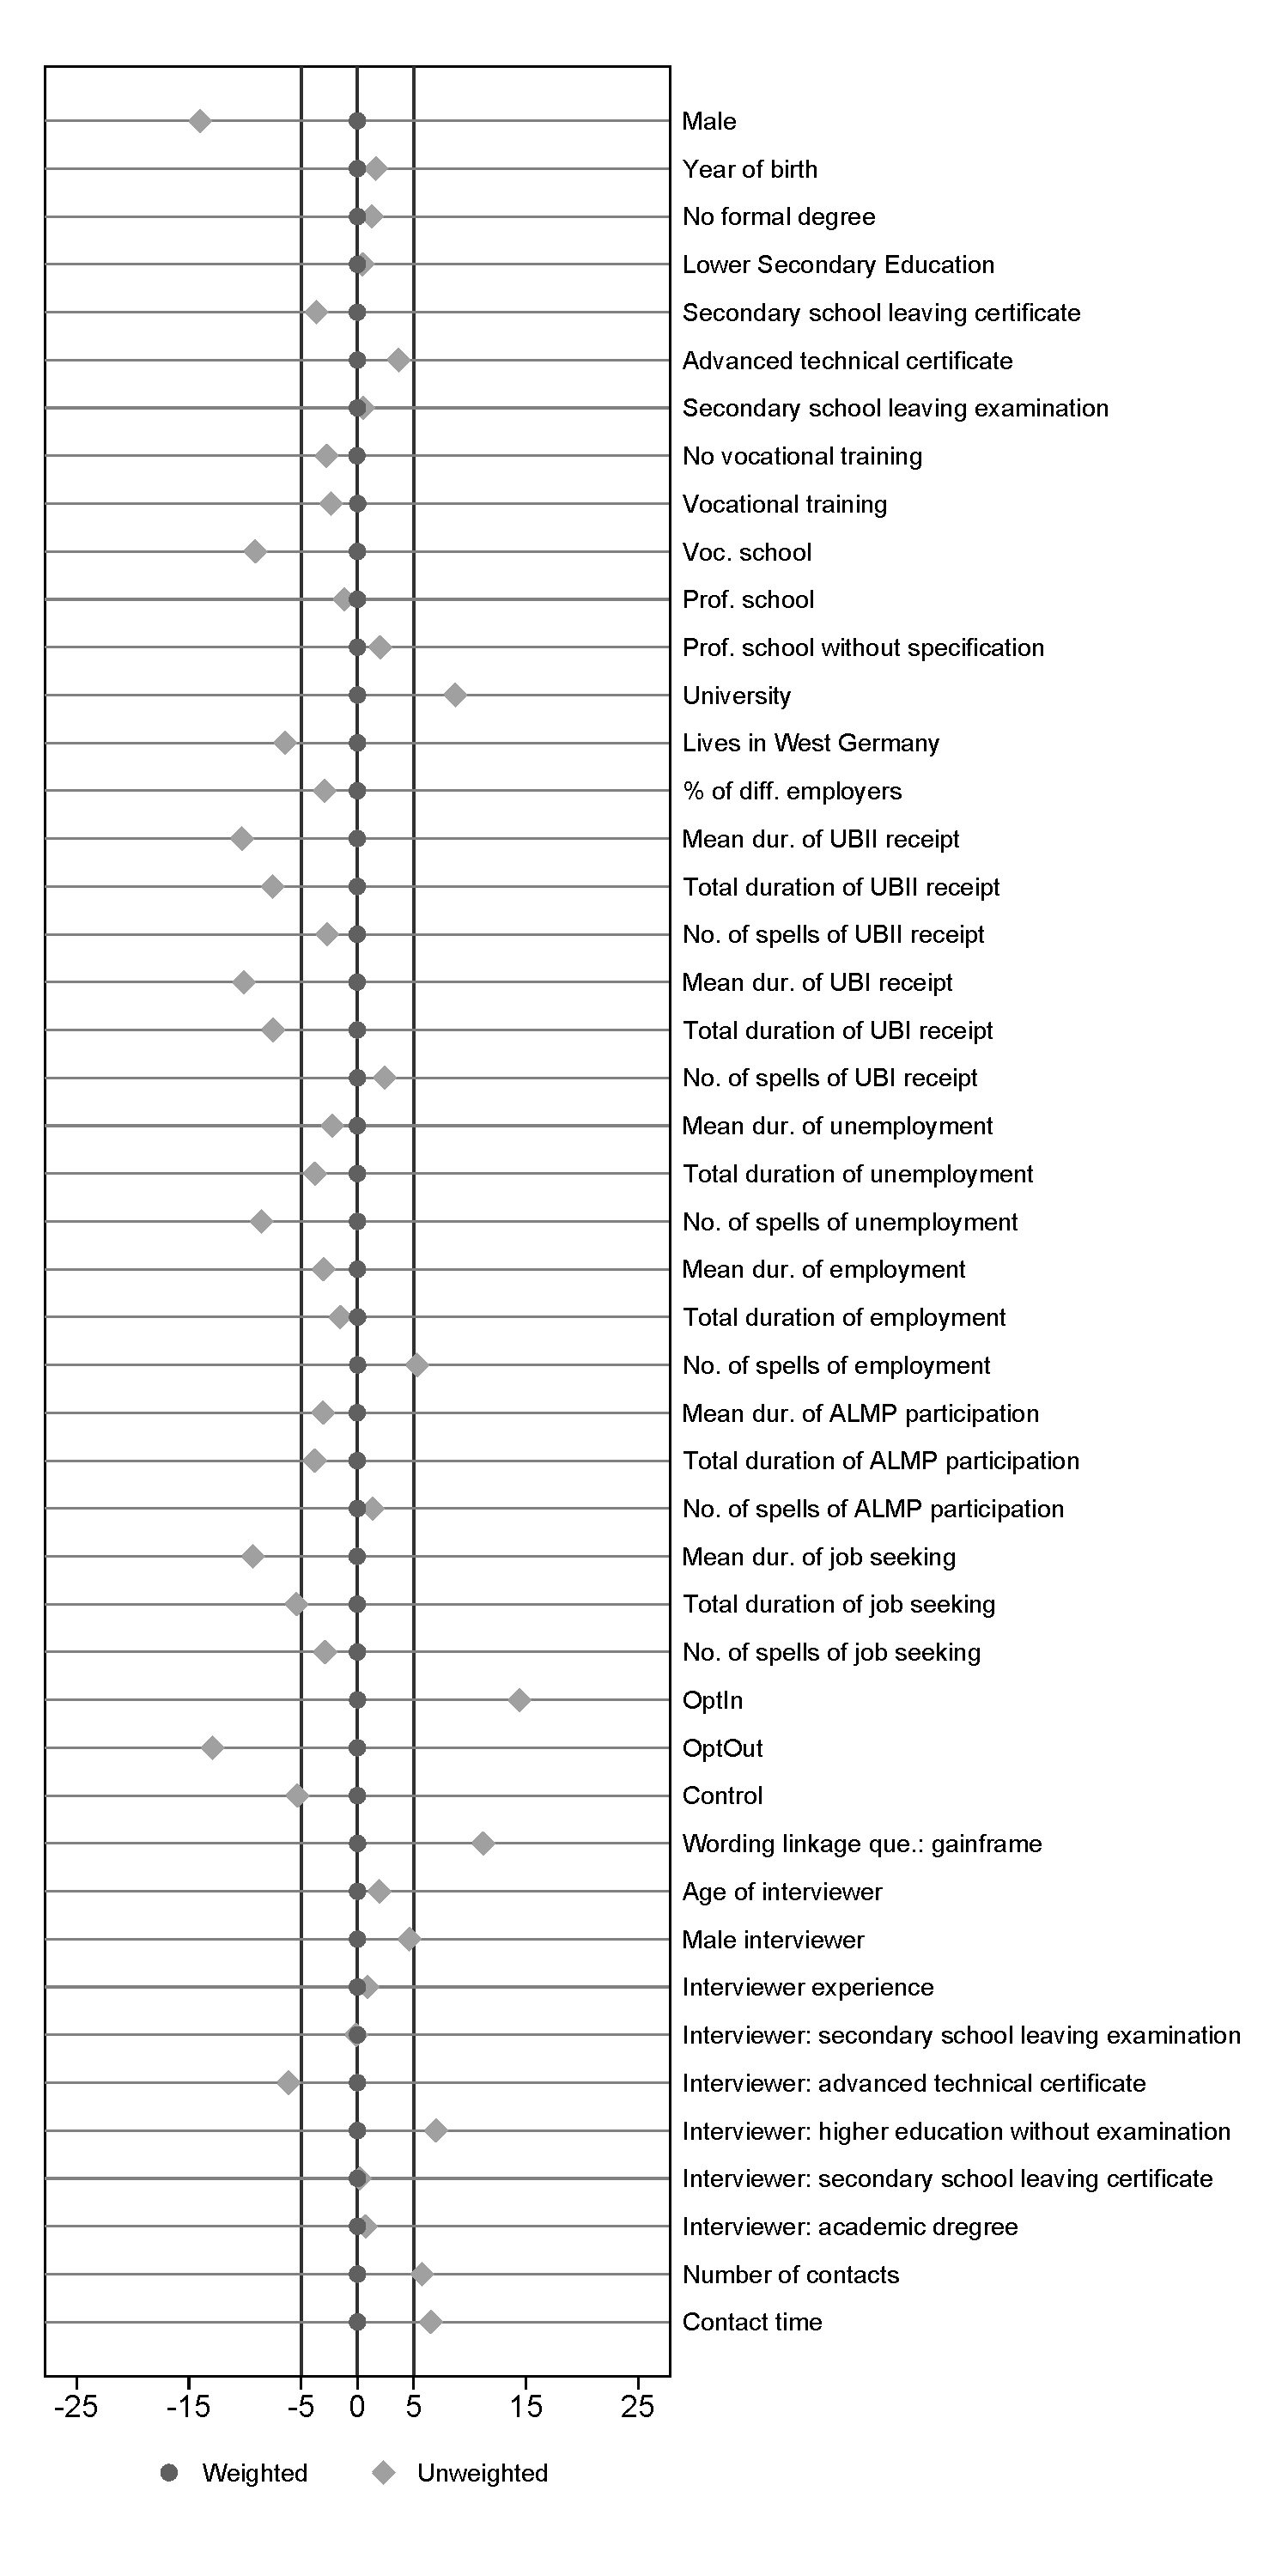
\includegraphics[scale=0.45]{balance.pdf}
% 	\label{fig:balance}
% \end{figure}

Unfortunately not all the analysis variables could be balanced out. Table \ref{tab:standardCATI} (p. \pageref{tab:standardCATI}) shows the 18 variables and the summarized standardized mean differences. The column of interest is the second: number of standardized differences \textgreater5 after weighting. As the guideline is that the standardized mean differences should be smaller than five (Caliendo and Kopeinig 2005) the entropy balance scheme failed for all variables that have at least one difference greater than five. In the end the employment variables from the second and third loop could not be balanced out with the entropy balance model. The same goes for the variables misreport in employment status for the respondents who stated non-employment in the first loop. Therefore I cannot calculate the average treatment effect for eleven of the 18 selected variables. 

The reason why the model did not work could be that the number of cases are insufficient as at the same time the differences in distribution over the discrete covariates are too big.  

A possible solution could be to stepwise take out the covariate with the highest standardized mean difference and include it to the regression model. In the next step the treatment effect could be analyzed in the context of the unbalanced covariates. The problem is that the share of unbalanced covariates is really high (see Table \ref{tab:standardCATI}) and therefore we would have blown up regression models. Further most of the covariates are not really interpretable as they were calculated to predict a propensity (see \ref{covar} Covariate for balance, p. \pageref{covar}).



\subsubsection{Treatment effect estimation for CATI variables}

In Table \ref{tab:emp_loop1} we can see the average treatment effects (ATE) that consent to the administrative data linkage question has on our selected variables. In contrast there is the estimation without the balanced covariates referred to as naive estimation. To get the average treatment effect and the naive estimation, a simple regression was used. Misreport in employment status is a binary coded variable (\(0=true\ report, 1=false \ report\)) Therefore we see the change of proportion that comes with the treatment. For example the average treatment effect of 0.03 is a change of three percentage points through the treatment of consenting to the linkage question at the beginning of the interview. That means that, due to the administrative data linkage question 20 (out of 669) more people misresport their employment status. As the standard error is as large as the estimate itself and the estimation can also be zero change in percentage points, the results are not significant and therefore the effect can be stated as coincidence. 

For the misreport in employment status we have an effect of three percentage points. This result does not change whether we use an estimation with balanced covariates or an unadjusted estimation. This suggests that balance is not necessarily needed for estimate the average treatment effect. 

If we take a deeper look and differ the misreport in employment status into the ones that stated that they have an employment and those who stated that they were non-employed, we can see that the treatment effect for the people who stated that they are employed decrease to one percent point for the balanced estimation and two percent points for the the naive estimation. Also we see that the standard errors are now bigger than the estimation itself and we can not make out a real direction of the treatment effect because the result can be in the negative and positive range. And also the non-significances show that there is no effect. 

It gets interesting as we look at the respondents who stated that they were unemployed. Unfortunately entropy balance failed to balance out the treatment and control group for this variable. We only have the naive result for interpretation. The effect we can see is quite large: 24 percentage points more of the respondents who consented to the administrative data linkage question at the beginning stated that they were non-employed even tough they had an employment. The result is even significant. It is really a strange result because it brings up the question why the respondents that got the administrative data linkage question at the beginning are more likely to state be non-employed even though they are employed. One possible explanation could be that side-jobs or mini jobs are not really considered as jobs. The same goes for the respondents who got the administrative data linkage question at the end though. Anyway, one of our hypotheses amounts that worse-respondents are more likely to satisfy in the response process. So the respondents could have ignored the instruction stating that side-jobs and mini-jobs are included as being employed and thought of his/her own definition of employment. 

This result can be seen as a support for the worse-respondent hypothesis since the measurement error increases with asking the administrative data linkage question at the beginning. There is a restriction though: we only have the naive estimation but not the estimation of the average treatment effect with balanced covariates. So this result could be a fluke. Also if it would be possible to balance out the covariates the effect should be smaller, because the overall misreport in employment status is exactly the same between the average treatment effect estimation and the naive estimation. The measurement error for the respondents who stated that they are employed differs only slightly from the overall misreport for both estimations. Also the average treatment effect estimate of the respondents who stated an employment is slightly greater than the naive estimation of the same group of respondents. So the average treatment effect for those who stated that they are non-employed has to be smaller than the naive estimation to gain the same average treatment for the overall misreport of employment status as the naive estimation for the overall misreport of employment status. Unfortunately this effect cannot be concretely measured in our case.

Table  \ref{tab:emp_loop1} also shows variables for the begin date of employment that the respondents stated. To remember dates is the hardest cognitive task a respondent is exposed to (Wagenaar 1986, Friedmann 1993). Our hypothesis is that worse-respondents should be less accurate about their estimate because they try to avoid cognitive effort or searching for the right month. Better-respondents should be more accurate. The linkage question should motivate them to search as long as they find the optimum date. The measurement error for the begin date of employment is calculated by the minimum deviation from the true month or the month from the administrative data. Also the deviation is measured as an absolute error, I do not decide between an under- or overestimate in the deviation. The average treatment effect is measured in months. That means with the consent to the linkage question at the beginning of the interview the deviation from the true date is about 1.8 months higher as if these respondents would had not consented to this question. Also the standard error has a high value of about 1.4 months and the effect is not significant. The naive estimation is slightly smaller as the average treatment effect estimation. Therefore balancing the covariates had a small effect. Again I cannot make out an effect. 

The last variable shown in Table \ref{tab:emp_loop1} is an indicator of whether the respondent choose to state the season instead of a month, did not know a month or just did not wanted to answer this question. Again this is a trigger for worse-respondents as they have an easy way out to answer this question. The effect is not strong (three percentage points), is not significant and therefore the treatment group does differ from the control group. 

Interestingly all the results in Table \ref{tab:emp_loop1} tell the same story. All effects are positive and suggest a shift of respondent behavior to worse-respondents because the measurement error increases with the administrative data linkage question at the beginning. But none (except for one naive estimate) are significant and we cannot prove a possible effect. It might be the case that the analysis does not have enough power and that with more observations an effect would be perceptible. 

Table \ref{tab:emp_loop2_3} shows the treatment effects of the second and third loop of the employment variables. Unfortunately only the naive estimations because the entropy balance method failed to balance the covariates for this variables. For the three employment status variables we see for both loops weak effects that are similar to the first loop in magnitude. With one exception they tell the weak story from the first loop in the reverse way. Under the hypothesis that we do not have enough power to prove an effect, this results suggest that after the first loop respondents turn out to be better respondents because measurement error is decreasing. But with the current data no such effects are perceptible. However, here the case base is even smaller. 

For the begin date, no differences between the respondents who consented to the administrative data linkage question at the beginning and those who consented to the same question at the end are found. The minimum deviation from the true date is -1.2 for the second loop and 0.24 for the third loop. The naive estimate of the effect is decreasing in absolute values might suggest that with enough power the differences between the groups are decreasing too. But it is rather the case that with each loop the minimum deviation from the date decreases\footnote{This an interesting point even though off-topic for this thesis. But it explains a paradox that is created by design and therefore is worth mentioning. Table \ref{tab:mean_dates_cati} (see Appendix \ref{tables}, p. \pageref{tab:mean_dates_cati}) shows the means of each minimum deviation of the begin date from each loop. The mean is decreasing with each loop and the differences between each loop are significant (see Table \ref{tab:t-test_date} in Appendix \ref{tables}, p. \pageref{tab:t-test_date}). I mentioned that with the increase of time it gets harder for the respondent to remember the date and accuracy decreases (Cannell et al 1981, Loftus et al 1992, Means et al 1989). Now we have a reverse result: the accuracy is increasing. That comes with the fact that respondents who stated a begin date before the 01.01.2010 were not forwarded to the next loop. So all respondents who had a begin date of employment that was long in the past were selected out for the next loops. Therefore in the first loop we have respondent with dates more far in the past that are harder to remember and therefore more prone for measurement error. With each loop the number of cases that  has a begin date of employment before 2010 decreases in proportion to the respondents who have a begin date after the 01.01.2010.}.  

The naive estimation for the variable that the respondents choose a season or declined to give an answer also shows no treatment effect.

In Table \ref{tab:inc_and_for} we see the average treatment effects and naive estimations for the variables income, Item non-response of income and citizenship. Income, as a sensitive item, should show us an effect because it might intrude the privacy of the respondents in another way then the linkage question does. But the results show no effect. The average treatment effect is 138.13 Euro, but the standard error is five times as big as the point estimate. Actually, the standard error increased from the naive estimation to the average treatment estimation. That could be a hint that the covariates for the entropy balance scheme were not appropriate \footnote{Many unrelated covariates could decrease the area of common support and increase the variance of the estimates (Bryson et al 2002, Augurzky and Schmidt 2000).}. 

For the item-nonresponse rate of income I cannot make out an effect either. But again, even though only slightly, the standard error increased with balancing.

There is no effect for the measurement error variable of citizenship too. This variable does not have a change between the average treatment effect and the naive estimation.  


\subsection{Results for web variables}

For the web survey I have five variables that I can analyze to check the better- and worse respondent hypotheses. For one I test the measurement error of the employment status between the respondents that consented in to the administrative data linkage question at the beginning and their counterfactual control group. The employment status is categorized in employed and non-employed. Unlike as in the CATI data I do not have cases that stated that they were non-employed. So I cannot test if the treatment effect between those who stated an employment and misreported and those who stated non-employment and misreported  is varying in the magnitude. Also I analyze the effect of consenting to administrative data linkage question on the deviation from the true begin date of the same employment. As dates are really hard to remember I also check the item non-response rate to see if the respondents who consented to the linkage question have less (better-respondents hypothesis) or more (worse-respondents hypothesis) item non-response. Further I also check the deviation and item non-response rate of the income. 

\subsubsection{Covariate balance for web variables}
Again we have different number of observations for each variable so that we need to apply the entropy balance model several times. I already showed in Figure \ref{fig:balance} how the standardized mean differences look like if the entropy balance scheme does his\textbackslash her purpose. In Table \ref{tab:standard WEB} we can see the summarized results of the balancing for each variable. The guideline to determine if the entropy balance scheme worked or not is the number of standardized mean differences less or equal five is zero. 



Unfortunately, Table \ref{tab:standard WEB} shows that the minimum deviation from the true begin date and the deviation from the true income have both greater or equal than eight standardized mean differences that are above five. The entropy balance scheme failed for these variables. Also we have a mean bias of 3.5 for the minimum deviation from the true date, we can not ensure balance. 



\subsubsection{Treatment effect estimation for web variables}
 
Table \ref{ATEwebemploy} shows the average treatment effects (ATE) that consent to the administrative data linkage question has on our selected variables. In contrast there is the estimation without the balanced covariates referred to as naive estimation. Again, simple regression models were used to get an estimate of the average treatment effect. 

For the misreport in employment status Table \ref{ATEwebemploy} shows an effect of -0.01. Compared to the constructed control group, consenting to the linkage question would lower the misreport in employment status by on percentage point. That means we have just about 5 less misreports for our sample of 469 respondents. This would support the better-respondent hypothesis, but since this result is not significant and the standard error is also really high we do not have a reliable result.    

Compared to the naive estimation the average treatment effect changes direction. Anyway, both results are not significant and show no effect. Concerning are the higher standard error by the average treatment estimation. This suggests that there are unrelated variables to the outcome or treatment assignment in the entropy balance model that increase the variance of the estimate. 
 


For the minimum deviation from the true month no balance was possible. Therefore only a naive estimation can be calculated. As we can see the deviation between the groups is 0.03 months. Consenting to the linkage question at the beginning has no effect on the accuracy with that respondents stated the begin month of their employment. 

The estimates of the item non-response indicator shown in table \ref{ATEwebemploy} are both non-significant and no effect is shown. Interestingly the point estimate changes from minus two percentage points that would support the better-respondent hypothesis, since item non-response decreases, to plus three percentage points that is supporting the worse-respondent hypothesis. It is again concerning that with balancing the standard errors of the estimation increase.   

Table \ref{tab:inc_and_for_web} shows the naive estimates of the deviation from the true income and the item non-response indicator for income. Also the Table shows the average treatment effect for the latter. Unfortunately the covariates for the deviation of income could not be balanced out and no average treatment effect can be calculated.

As hypothesized the income as a sensitive question should either increase the effect of worse-respondents or decrease the effect of better-respondents. The naive estimation show in Table  \ref{tab:inc_and_for_web} does not show any effect that could support one of our hypotheses. 

For the item non-response variable  I cannot make out an effect either. Both estimates are near to zero and not significant. Again we have higher standard errors for the average treatment effect and therefore a hint for a misspecified entropy balance model. Similar to the item-nonresponse indicator of the begin date the point estimates change directions and would support, if significant, different hypotheses. Still in this case the average treatment effect estimation would support the better-respondent hypothesis and the naive estimation the worse-respondents hypothesis.  

All results in this section show no evidence for either one of the both hypotheses. I cannot make out a pattern that suggests anything. The only thing result is that the standard errors increase with the average treatment estimation.

\subsection{Comparing the results of the CATI and web analysis} 

In both datasets no supports for the better-respondents that should have lower measurement error and item non-response rates or worse-respondents that should have higher measurement error and item non-response rates were found. Except for one naive estimate in the CATI analysis. This naive estimate shows a effect from consenting to the linkage question on the misreport behavior of the respondents when they stated that they were non-employed. An average treatment estimation was not possible because of the failed entropy balance model for this variable. Further I cannot check and compare this result for the web data because we only have respondents who stated that they were employed. 

If we compare the results of the average treatment effects from CATI and web, we can see in the web survey that with the average treatment estimations have increased standard errors compared to the naive estimation. In the CATI data the standard errors only slightly increase with the average treatment estimation. This suggests that the entropy balance model might be misspecified, with a higher impact in the web data. This comes probably through the fact that in the CATI data additional variables (interviewer and record call data) incorporated that can lower the variances. 

If we compare Table \ref*{tab:standardCATI} (see p. \pageref*{tab:standard WEB}) with Table \ref*{tab:standard WEB} (see p. \pageref*{tab:standard WEB}), it seems like in the CATI data the entropy balance works pretty or in no sense. Every time when balance is achieved the standardized differences go not over 0.1. In the web survey the entropy balance model does not achieve such good results. The standardized mean differences stay less or equal five, but scatter more in the range of five and zero than in te CATI data. This suggests that the selection bias between consenters in the begin and end is higher in the web survey.

\section{Summary and Discussion}

The purpose of this thesis was to find out, if asking for linkage consent at the beginning leads to higher or lower measurement error. I hypothesized that the administrative data linkage question has an effect on the response behavior of the respondents, brought about by interpretations the respondents might have about consenting. By consenting respondents give permission to link survey data with administrative data. Therefore they could believe that their answers may be checked after executing the interview. I hypothesized two possible interpretations respondents may have from this belief. For one, the respondents could believe that they get in trouble for not reporting the true value of the asked question. So they may make an effort to give better answers: better-respondent hypothesis. On the other side the respondents could think that their reports can be corrected after the interview and therefore care less about answering questions: worse-respondent hypothesis. With better-respondents, studies which ask for linkage at the beginning would get more accurate results for respondents who consented. If the linkage question leads to worse-respondents, studies have to deal with higher measurement error when choosing to maximize linkage consent. 

To tackle the hypotheses I used a CATI and a web dataset. Each of these surveys contained an administration data linkage experiment: one set of respondents was asked at the beginning and one at the end. I compared the consenters from the linkage question at the beginning with their counterfactual group constructed from consenters of the linkage question at the end and estimated an average treatment effect. If I had just compared the consenters from the beginning with the consenters from the end, the results would be rather naive because the analysis would suffer from selection bias. In order to not have the analysis corrupted by confunding factors, we need a random assignment of the respondents to the group that received the treatment and the group that did not. For that I used an entropy balance model to obtain weights that adjust the control group so that it is balanced with the treatment group. 

The items of interests were several measurement error variables and item non-response variables.

The analyses in this thesis reveal that the administrative data linkage question has no effect on the response behavior. All results of the average treatment effect estimation were non-significant. There is no effect on the measurement error variables and no effect on the item non-response variables that were analyzed. The reason for that may be ascribed to shortcomings of this study. Anyway, this finding is good news for studies that already worked and will be working with linked data that got permission for linkage through a linkage question asked at the beginning of the survey. 

There is limitation to this statement because I found that consent to the linkage question at the beginning has an effect on the share of misreports for respondents that stated non-employment even though they were employed. Unfortunately I only have a naive estimate since the entropy balance model did not work for this variable.

It is also possible that the null findings in this study are due to shortcomings in the data sets. For one we have a huge loss of cases before the analyses had even started. I had to drop non-consenters, wrong matches, incompletes, officials and self-employed persons because no information was available for those groups or they could have corrupted the analyses. Due to that decision the analysis lost around 24\% of cases for the CATI and around 46\% of cases for the web survey meaning a loss of power. 

To construct the counterfactual group an entropy balance model was used to gain weights that equal the distribution between the treatment and control group. Trying to satisfy the strong ignoreabilty assumption which is not fully testable, I used the kitchen sink approach, which advocates including all variables (Eckman and Nichols 2015). Unfortunately, a large number of available variables (including all variables from the survey) that were observed could not be taken for this model because they were corrupted by the treatment variable itself. Only the variables from the administrative data (and interviewer and call record data for the CATI dataset) could be used. It is a debatable point whether these variables are enough or do not account for all distribution inequalities between both groups. The increasing standard errors between the average treatment effect and naive estimation in some results suggest that the model has some variables that are not related to the treatment assignment. As a consequence the variance increases which leads to an increase of standard errors (Stuart 2010). In this case the kitchen sink approach might not be the best choice.

Further, the treatment and the control group could not be balanced out for each analysis variable. The reason for that may be that the number of cases is too small while differences between the groups are too large. Therefore the entropy balance model fails in some cases. 

If the entropy balance model is not defined in the right way, our assumption about randomly distributed groups does not apply. Meaning that the assumption that the average treatment effect of the treated equals the average treatment effect does not hold anymore. In this case it is even debatable if an average treatment effect of the treated is estimated. In this case I would not have calculated an average treatment effect but a biased naive estimation. 

I hypothesized that the consent to the linkage question either leads to better-respondents or worse-respondents. But it may be possible that both hypotheses canceled each other out. In the background section I mentioned the Optimizer-Satisfier-Continuum on which each respondent has an initial location. I hypothesized that with the consent to the linkage question they move on this continuum either to the optimizer or to the satisfier side. It is possible the linkage question has the effect that some respondents move to the optimizer side and others move to the satisfier side. This phenomenon could also explain my null results.

In this study, only respondents that consented to the administrative data linkage question could be analyzed. I cannot ensure that these conform to a population we can make inference to. I balanced the treatment and control group. There is no adjustment to the population of the Integrated Employment Biographies which the data is sampled from or a population like the German society. Therefore significant results can only make an inference to a population that has the same design as this study. How reasonable this inference is left to the reader. 

Further I cannot make any statements for non-consenters. Maybe the administrative data linkage question has an effect on the response behavior and our hypotheses apply to that. But that cannot be tested because non-consenters cannot be linked to administrative data\footnote{In fact there is one study that overcomes this restriction: Sakshaug and Kreuter 2012.}.

Who consents and who does not depends on survey topic and design of the study. 
We want to ask for linkage at the beginning of the interview because that gives the highest consent rates but we worry that the linkage question changes the behavior of the respondents in a way that they make less effort in answering the survey questions. The results of this study suggest that we do not have to worry about that. Anyway, several studies found different characteristics between consenters and non-consenters. The results cannot easily be transferred to other studies and have to be viewed in the specific design of this study. Therefore the result that the administrative data linkage question does not have an effect on the respondents do not have to apply for other studies that asked for administrative data linkage. 



\section{Filename convention}

All files should be renamed such that the XXXX in the filename becomes
the entry number. If the entry number is XXXX,

\bci
\item Title, abstract, etc. should be stored in  \texttt{XXXX\_header.tex}
\item The article should be stored in \texttt{XXXX\_artcl.tex}
\item Table 1, Table 2 $\ldots$ Table K, should be stored in
  \texttt{XXXX\_tab1.tex}, \texttt{XXXX\_tab2.tex} $\ldots$
  \texttt{XXXX\_tabK.tex} 
\item The Bibliography is created with BibLatex (Biber) from a BibTex
  file in \texttt{XXXX\_bib.bib}
\item Figure 1, Figure 2 $\ldots$ Figure K, should be stored in
  \texttt{XXXX\_fig1.tex}, \texttt{XXXX\_fig2.tex} $\ldots$
  \texttt{XXXX\_figK.tex} (if any)
\item The appendix should be stored in \textrm{XXXX\_appendix.tex} (if
  any) \eci

\section{Typesetting rules}

We follow the rules of the APA Publication Manual. Most of the rules
are implemented thru srm\_main.tex, but please


\bci
\item do not use bold face in the text body
\item do not use vertical lines in tables
\item do not use italics for proper english words in equations should.
\item use identical symbols for math symbols in the text body and in equations
\item take care that separators, hyphen, minus-sign differ in
  length. Look -- as an example -- on on the minus-sign in the equation $1-1=0$
\item prevent parentheses in parentheses in the text body; 
\item use ``double quotation marks''. The rule is: ``We use `single
  quotation marks' only inside  double quotation marks''.
\eci

If in doubt  refer the the APA publication manual, 6th edtion.


\section{Section headings}

We use sections, subsections and subsubsections. Not
more. Never. Unlike APA 6, we we number sections and subsection. The
file \texttt{srm\_main.tex} does this automatically.

\section{Itemize and Enumerate}


Itemlist are typesetted with the ``APAitemize''
environment. Enumeration is typesetted with the ``APAenumerate''
environment. The former can be started/closed with the LaTeX commands
``bci'' and ``eci'', while the latter can be started/closed with
``bce'' and ``ece''. Example. The code

\begin{scriptsize}
\begin{verbatim}
\bce
\item bla bla
\item more bla bla
\ece
\end{verbatim}
\end{scriptsize}

creates this

\bce
\item bla bla
\item more bla bla
\ece

\section{Tables}

Tables are typesetted in a table environment or table* environment --
depending on the size of the table. The table* environment is for wide
tables. Inside the table we allways use threeparttable as shown in the
code below:

\begin{scriptsize}
\begin{verbatim}
\begin{table}
  \begin{threeparttable}[b]
  
  
  
    \caption{The caption of the table}
    \begin{tabular}{l.{2}.{2}}
      \toprule
      Left aligned header & \mc{numheader 1} & \mc{numheader 2} \\ 
      \midrule
      Two digit numbers & 1.34 & 0.20\tmark{a} \\
      More two digit numbers & 1.50 & 1.23 \\ \midrule
      Zero digit number & \mc{300} & \mc{300} \bottomrule
    \end{tabular}
    \vspace{.5em}
    \begin{tablenotes}\small
    \item We start with a general footnote, if any. Note that we don't
      want too many signficance stars.
      
    \item [a] A footnote for footnote signs. Significance footnote
      come last.
      
    \item $*$ p<0.05
    \item $**$ p<0.01
    \item $***$ p<0.001


    \end{tablenotes}
  \end{threeparttable}
\end{table}
\end{verbatim}
\end{scriptsize}

Which leads to Table 1.

\begin{table}
  \begin{threeparttable}[b]
    \caption{The caption of the table}
    \begin{tabular}{l.{2}.{2}}
      \toprule
      Left aligned header & \mc{numheader 1} & \mc{numheader 2} \\ 
      \midrule
      Two digit numbers & 1.34 & 0.20\tnote{a} \\
      More two digit numbers & 1.50 & 1.23 \\ \midrule
      Zero digit number & \mc{300} & \mc{300} \\ \bottomrule
    \end{tabular}
    \vspace{.5em}
    \begin{tablenotes}\small
    \item We start with a general footnote, if any. Note that we don't
      want too many signficance stars. 
      
    \item [a] A footnote for footnote signs. Significance footnote
      come last. 
      
    \item $*$ $p<0.05$
    \item $**$ $p<0.01$
    \item $***$ $p<0.001$
    \end{tablenotes}
  \end{threeparttable}
\end{table}


%%% Local Variables: 
%%% mode: latex
%%% TeX-master: "srm_main"
%%% End: 



\section{Figures}


Figures must be provided as scalable vector graphs, EPS or
PDF. Figures are included in the article as follows:

\begin{verbatim}
\begin{figure}
  \centering
  \includegraphics[width=\linewidth]{XXXX_fig1}
  \caption{The caption as provides by the author}
\end{figure}
\end{verbatim}

\section*{Acknowledgements}

Acknoledgements comes last. They are typsetted with the starred
version of section, i.e. 

\begin{verbatim}
\section*{Acknowledgements}
\end{verbatim}

\section{Bibliography}

We use Biblatex for the Biobliography. You can find the full
descritpion of BibLateX on the internet, but examples for the the main
functions are shown below:

\bci
\item The normal cite is for citations without parentheses. Example:
  \cite[see][pg.\,12]{carrasco03}
\item parencite is for citations in parentheses. Example:
  \parencite[see][pg.\,12]{dept10}
\item textcite if for text citations. Example: 
  \textcite[see][pg.\,12]{dorer11}.
\item For special situations there are also the parencites and
  textcites commands. Here is an example with parencites: 
  \parencites(See)(and the
  introduction)[35]{fitzgerald11}[78]{dorer11}[23]{goerman07}. See the
  BibLatex manual for details. 
\eci

Note that you must use the command ``biber'' to create the actual
Bibliography instead of bibtex. 



%%% Local Variables: 
%%% mode: latex
%%% TeX-master: "srm_main"
%%% End: 
